\documentclass[UTF8]{ctexart}
\usepackage{subfigure}
\usepackage{caption}
\usepackage{amsmath}
\usepackage{amssymb}
\usepackage{pifont}
\usepackage{geometry}
\usepackage{graphicx}
\usepackage{gensymb}
\usepackage{wrapfig}
\usepackage{titlesec}
\usepackage{float}
\usepackage{diagbox}
\usepackage{fancyhdr}
\usepackage{color}
\pagestyle{plain}
\geometry{a4paper,scale=0.8}
\CTEXsetup[format+={\raggedright}]{section} 
\title{通网2014-2015期末}
\author{Deschain}
\titlespacing*{\section}
{0pt}{0pt}{0pt}
\titlespacing*{\subsection}
{0pt}{0pt}{0pt}
\titlespacing*{\paragraph}
{0pt}{0pt}{0pt}
\titlespacing*{\subparagraph}
{0pt}{0pt}{0pt}
\titleformat*{\section}{\normalsize}
\begin{document}
\maketitle
\section*{一、填空题}
1.设X为7元离散信源,其概率分布为
$\begin{pmatrix}
    x_1         & x_2          & x_3          & x_4         & x_5          & x_6          & x_7 \\
    \frac{2}{7} & \frac{1}{14} & \frac{1}{28} & \frac{2}{7} & \frac{1}{14} & \frac{1}{28} &
    \frac{3}{14}                                                                                \\
  \end{pmatrix}$,携带信息量最大的符号为(\quad\quad\quad);该信源的熵值为(\quad\quad\quad),
7元离散信源的最大熵为(\quad\quad\quad)。\\
2.某个线性分组码记为(23,12,7)码,其信息位长度为(\quad\quad\quad),编码长度为(\quad\quad
\quad),基本校验矩阵行数为(\quad\quad\quad),最小码距为(\quad\quad\quad),如果全部用于纠错,
可以纠(\quad\quad\quad)位错,如果全部用于检错可以检(\quad\quad\quad)位错,如果试图纠正任意的
1位错,还可以同时检(\quad\quad\quad)位错。\\
\section*{二、简答题}
1.均匀量化和非均匀量化各适用于什么样的信源?他们各自存在什么样的特点?\\
2.简述时分复用(复接)的基本概念、主要困难和解决方法。\\
3.请简述拥塞控制的方法。为什么网络月拥堵,少许增加业务到达率所引起的等待延时越大?请尝试举例定
量化说明。\\
\section*{三、计算题}
1.某信源输出随机变量X,其概率密度函数如图1所示,量化分层电平分别设在$-\frac{2}{3},\frac{2}{3},
  \frac{4}{3},2$,计算:(每小题5分)\\
(1)该量化器的信噪比;\\
(2)若用0、1bit表示量化器的输出,计算最短平均码长。\\
\begin{figure}[H]
  \centering
  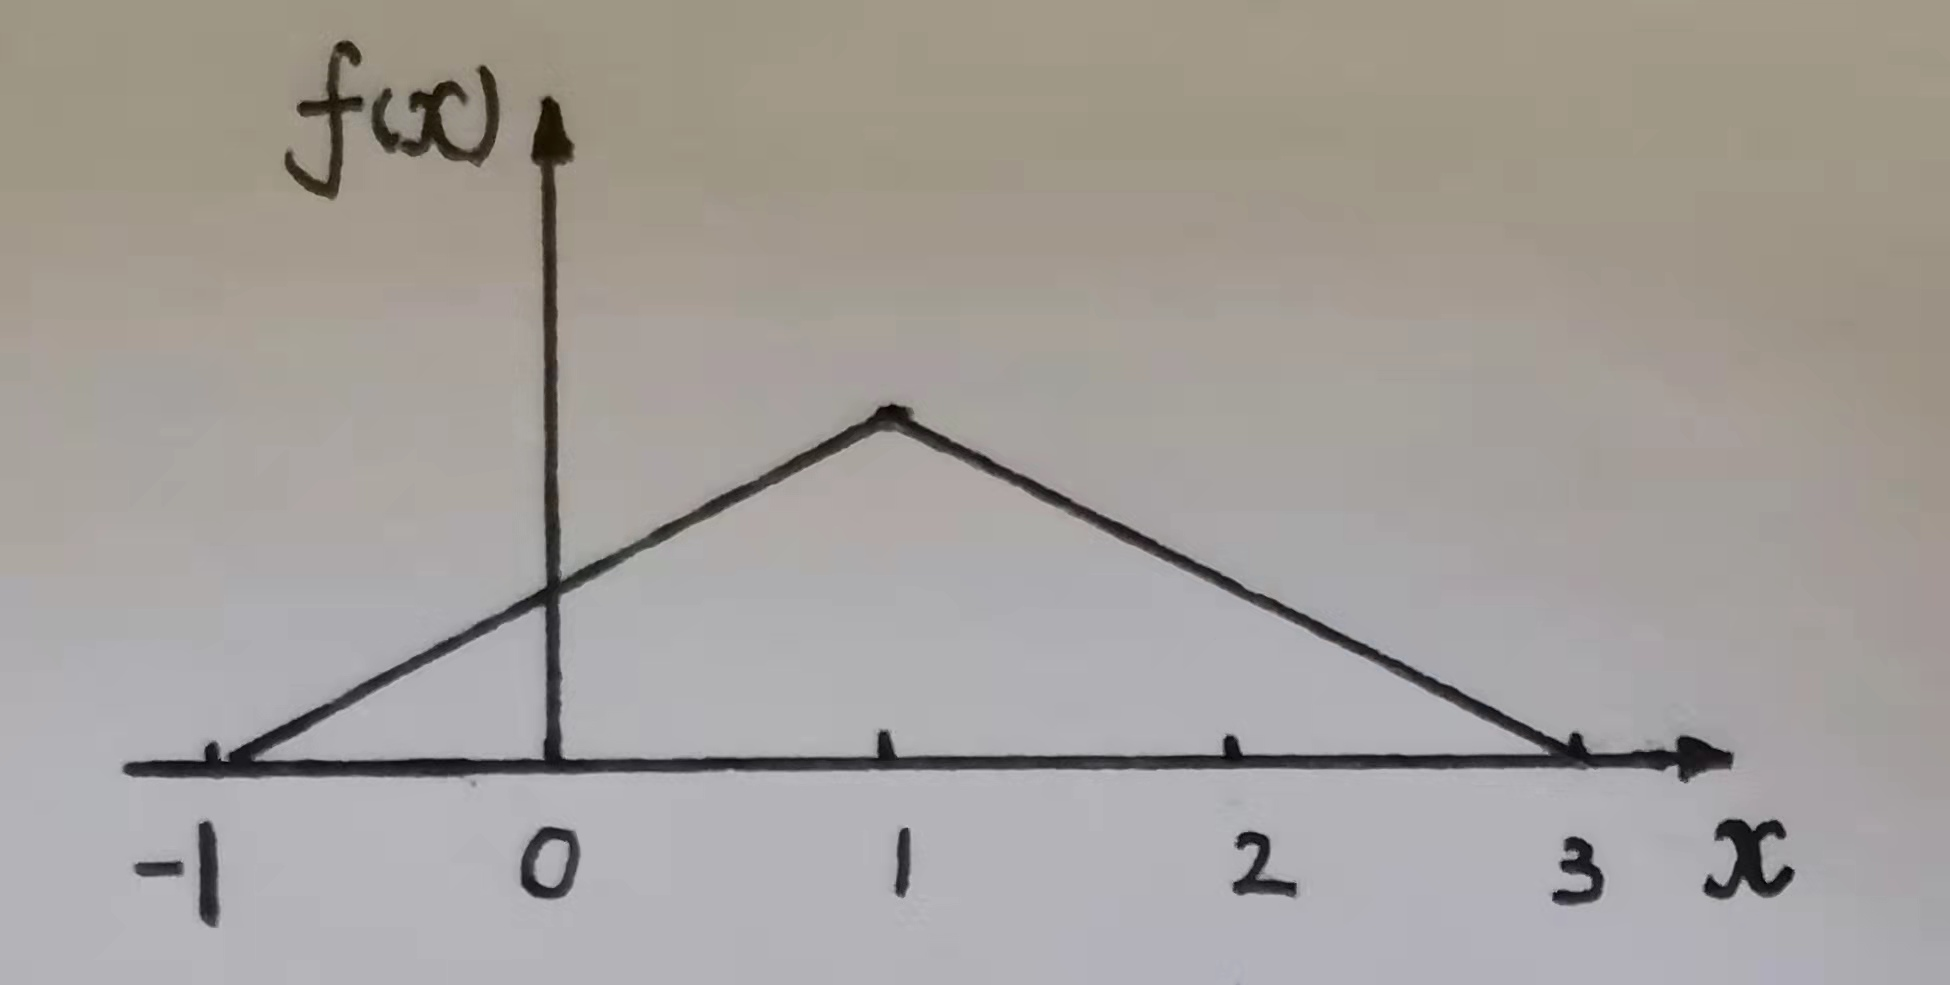
\includegraphics[width=5cm,height=3cm]{3_1.jpg}
  \caption*{图1}
\end{figure}
2.某线性分组码的生成矩阵为:$G=
  \begin{bmatrix}
    1 & 1 & 1 & 0 & 0 & 1 & 0 \\
    1 & 0 & 1 & 1 & 1 & 0 & 0 \\
    0 & 0 & 1 & 0 & 1 & 1 & 1 \\
  \end{bmatrix}$\\
(1)求编码输入全“1”时,编码后的码组;\\
(2)请将它转换成信息位在前,校验位在后的系统码生成矩阵;\\
(3)求它的一个监督矩阵;\\
(4)其码组长度为多少,监督位长度为多少;\\
(5)若接收码组为0111110,求校正子,及最可能的发送码组。\\
3.卷积码编码器如图2所示,试回答如下问题:\\
(1)画出状态图、网格图。\\
(2)计算输入bit序列01001101110……(省略号为全0)的编码输出;\\
(3)若接收到bit序列为100\quad101\quad011\quad101\quad110\quad000……(省略号为全0),用Viterbi
算法计算译码结果。\\
\begin{figure}[H]
  \centering
  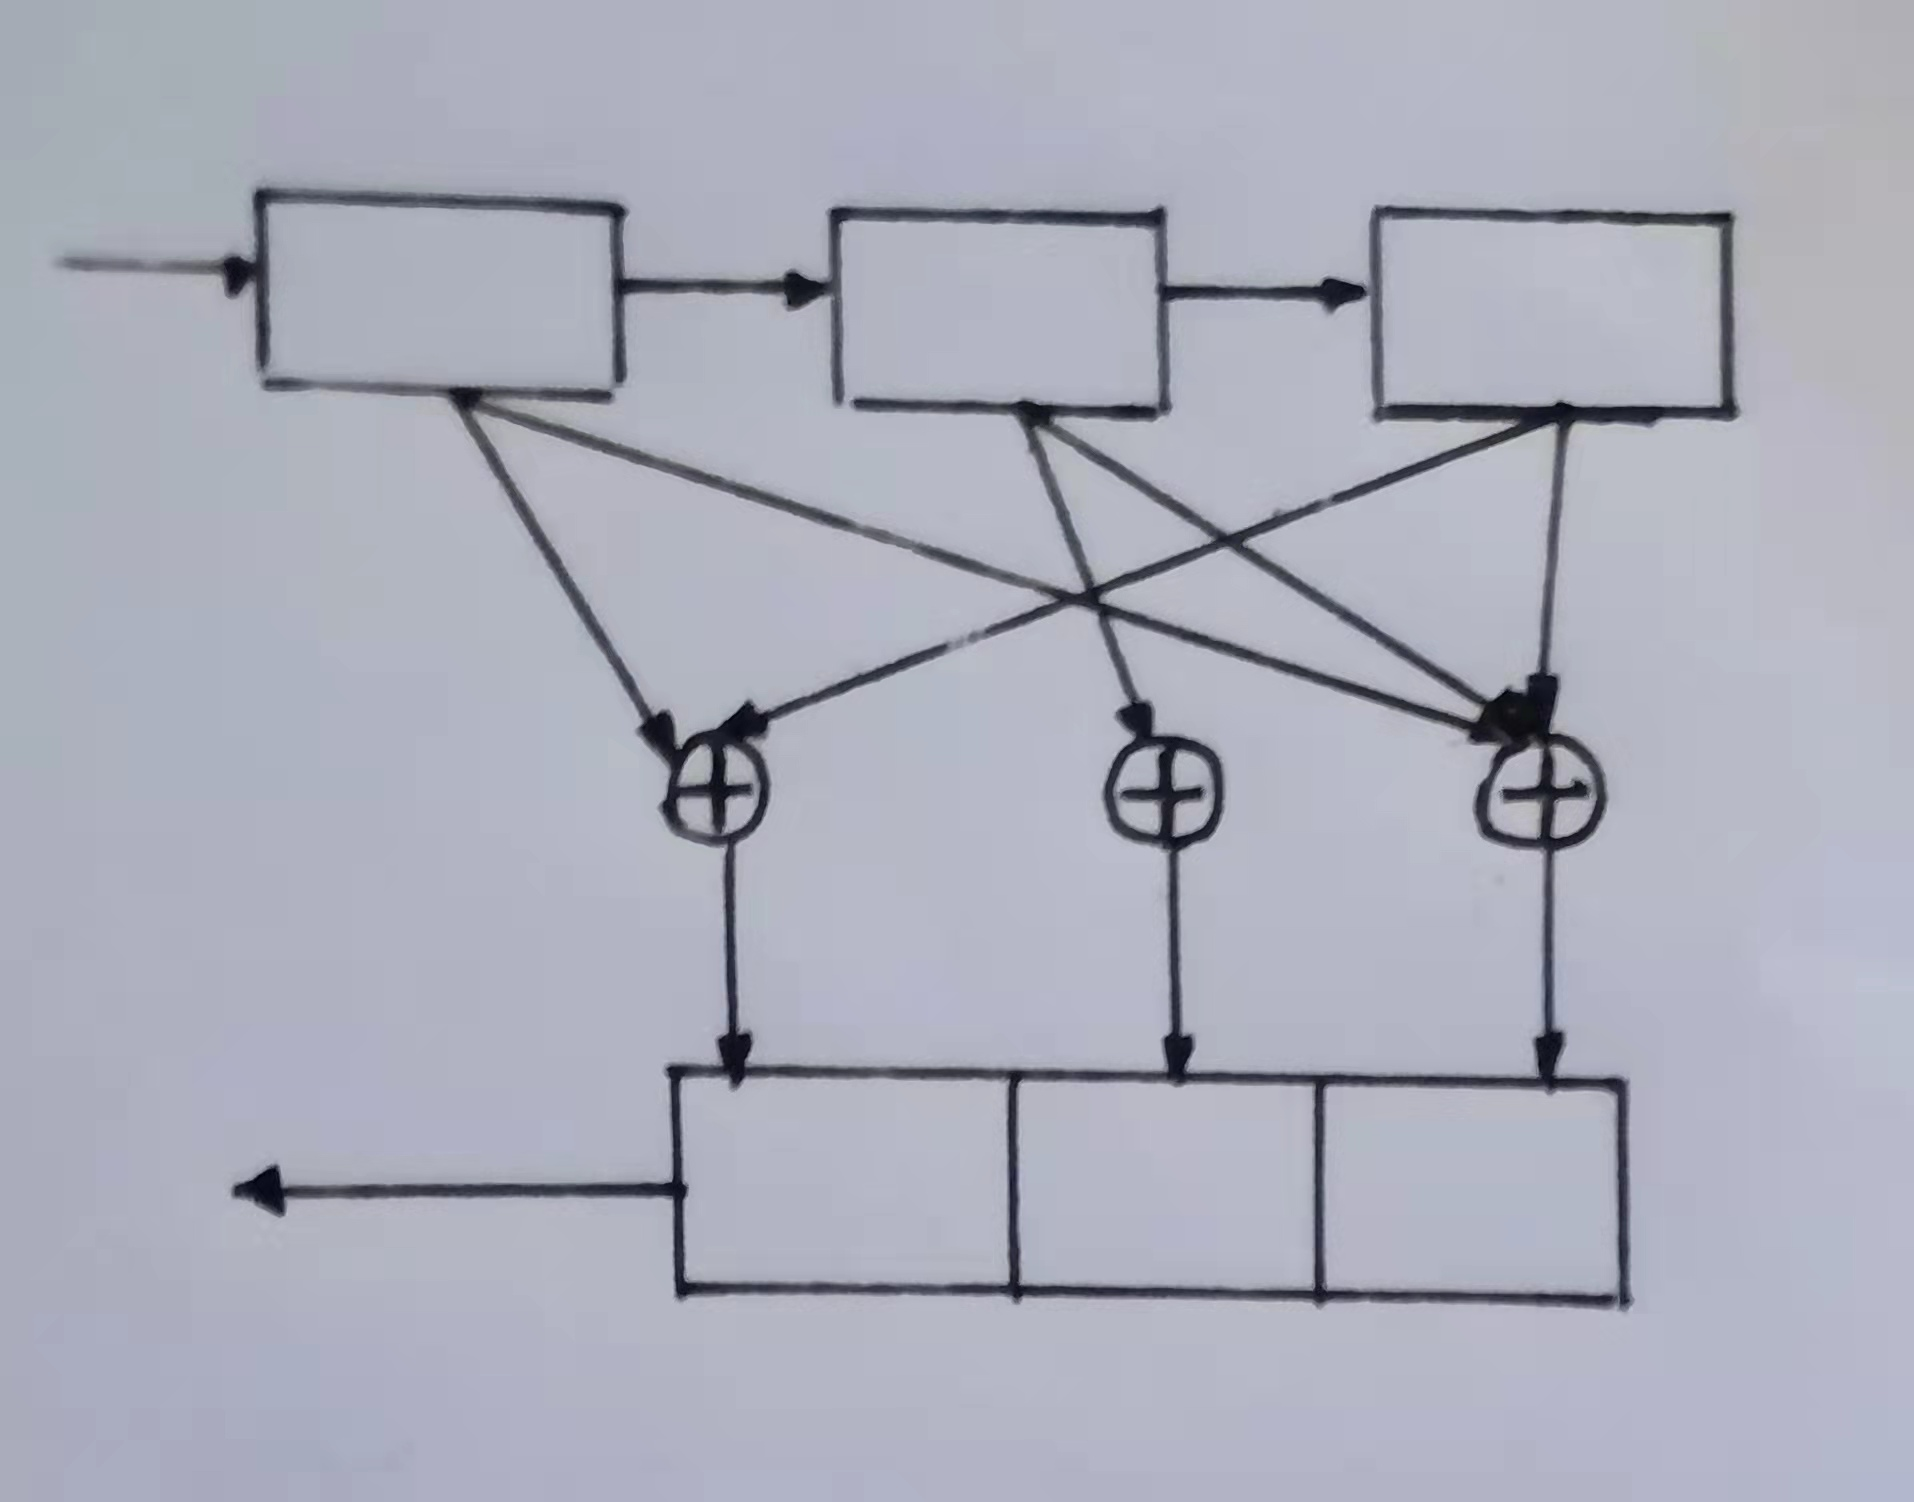
\includegraphics[width=3cm,height=3cm]{3_3.jpg}
  \caption*{图2}
\end{figure}
4.图3给出一种网络拓扑结构,每条边的代价均已标出,请计算图中从S到D的最佳路由,需讨论最佳路径随
非负实数x和y取值的变化。(提示:可采用Dijkstra算法)
\begin{figure}[H]
  \centering
  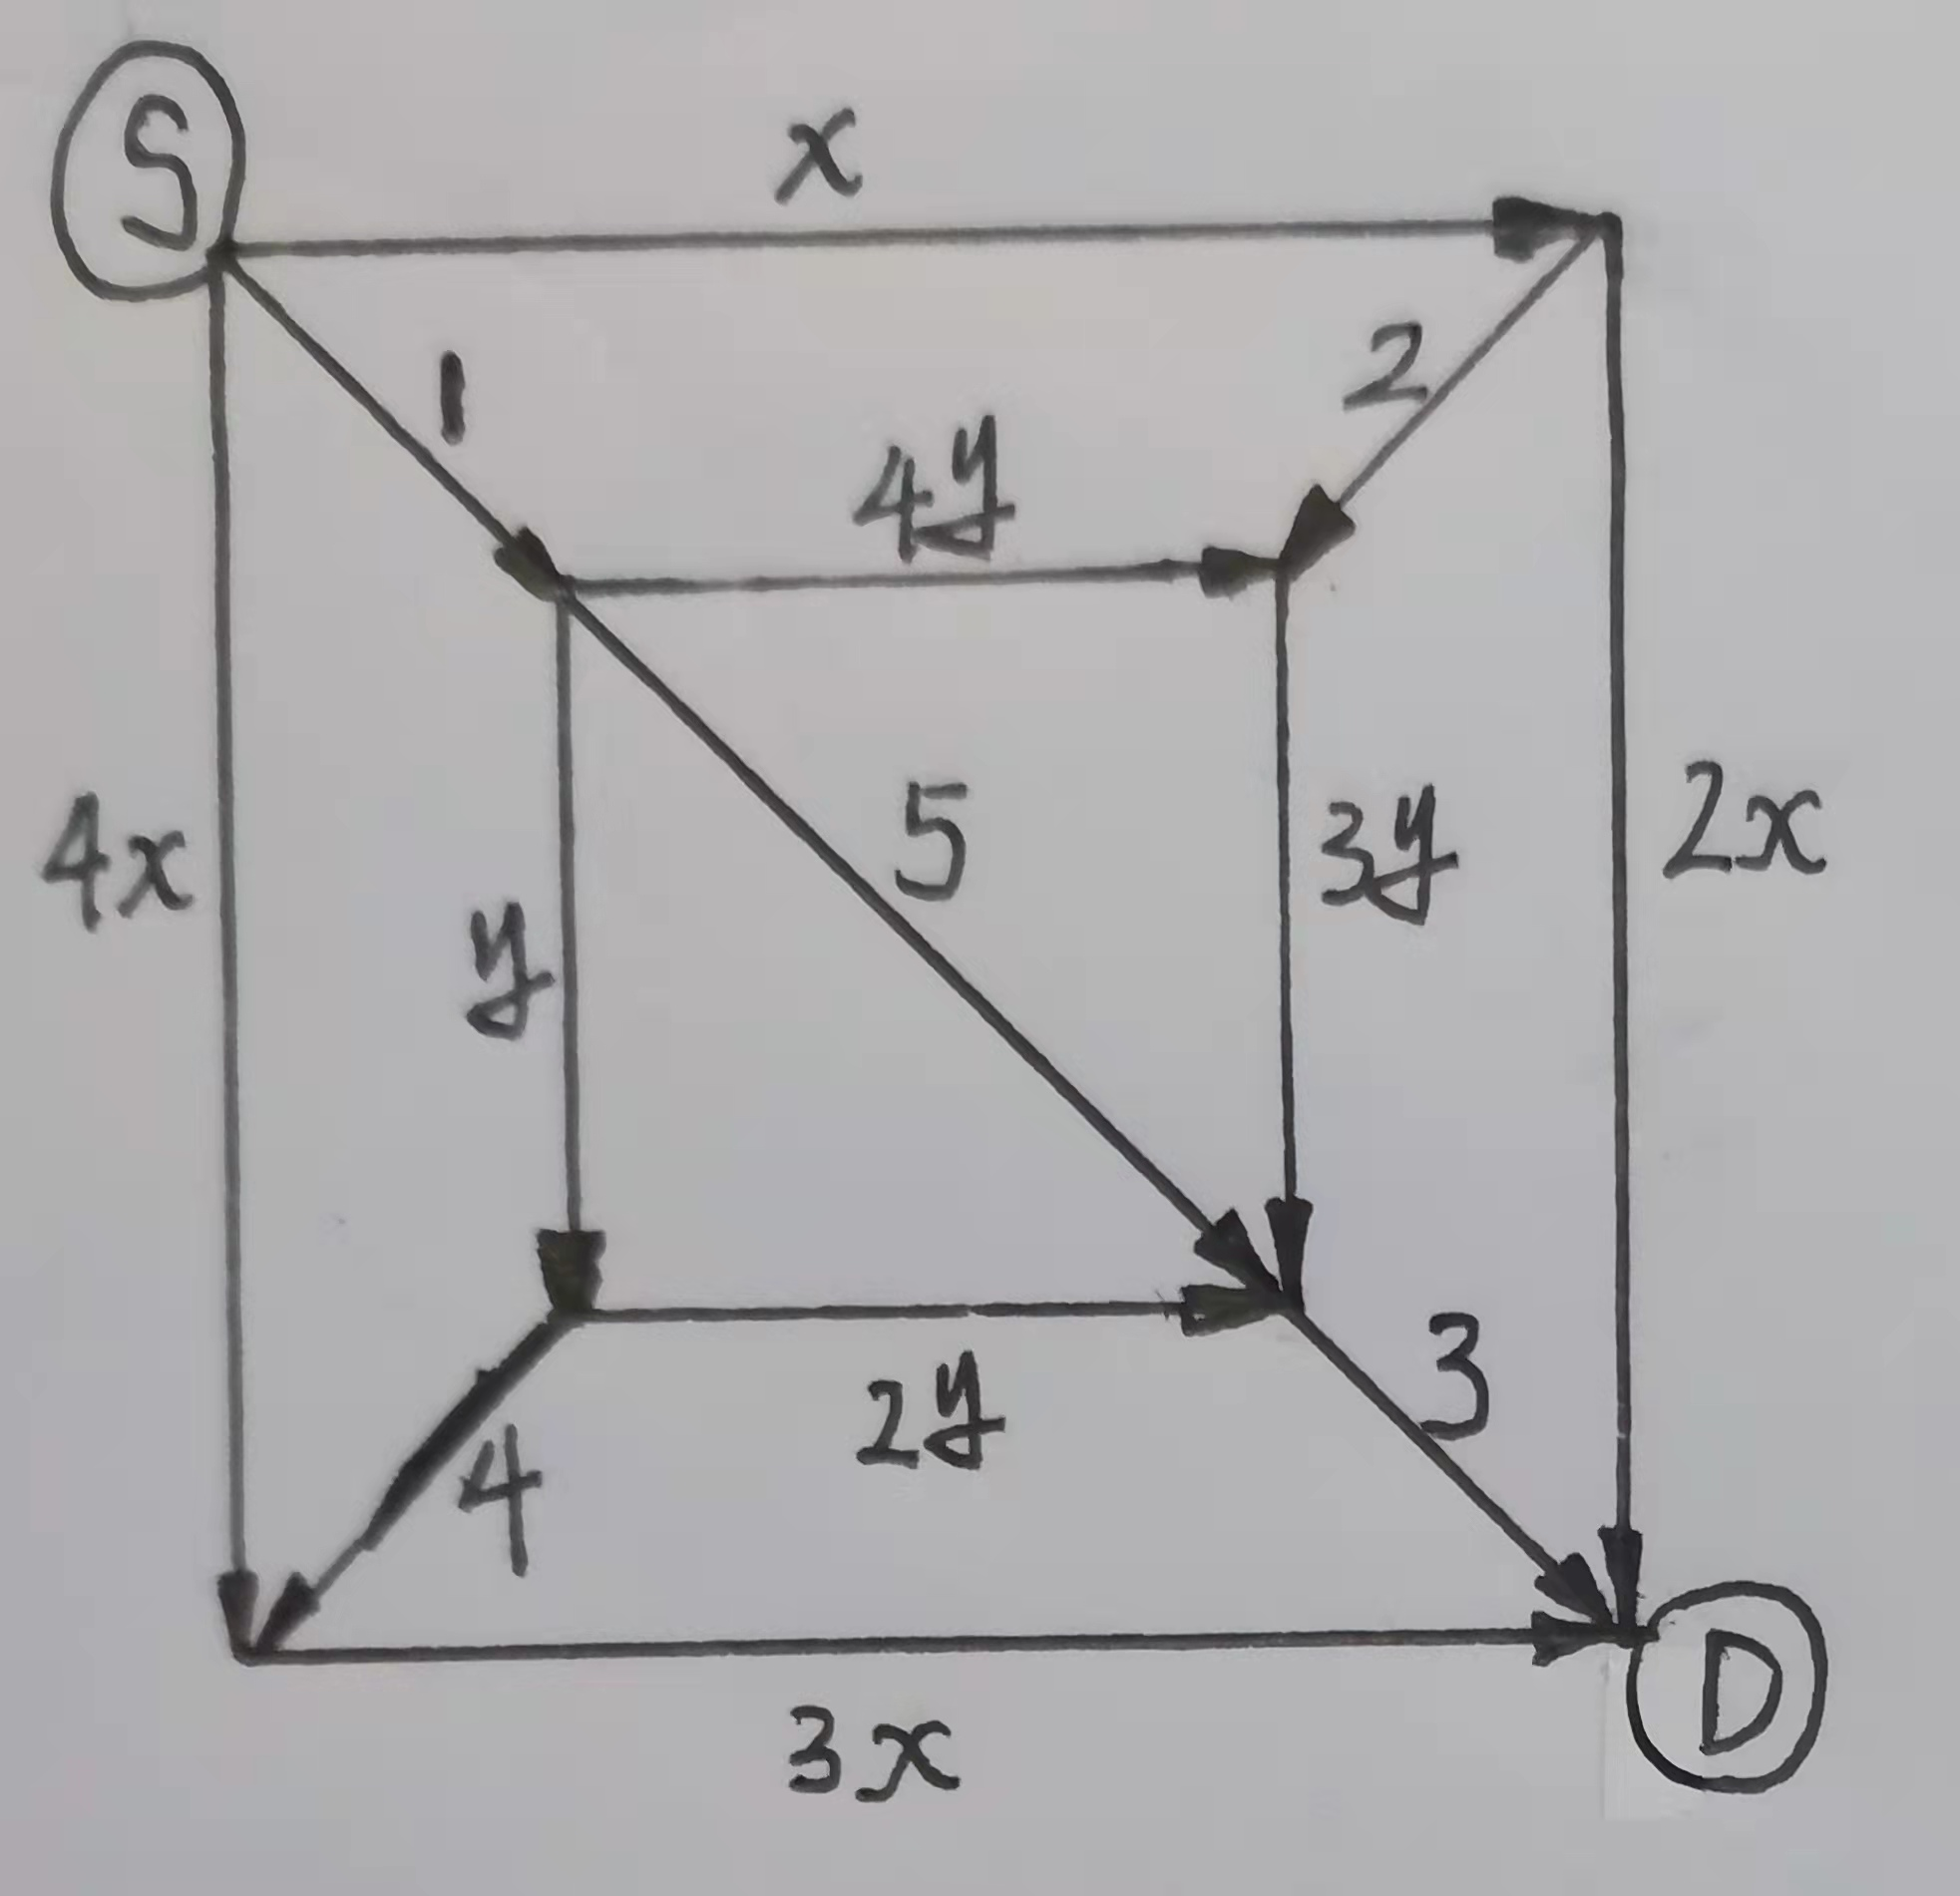
\includegraphics[width=4cm,height=4cm]{3_4.jpg}
  \caption*{图3}
\end{figure}
5.某两点之间的电缆载波通信系统,信源数据率为32kps,进行16QAM调制,发送的成形滤波器频响为
$\alpha=0.5$的根号升余弦,载波频率为100kHz,试回答以下问题(写出求解过程,前面问题答不出来
可以作一定的假设以后继续做下一问题)\\
(1)画出调制星座图;\\
(2)调制后的符号率是多少?以全部信号带宽为准,占用多少带宽?整个系统的总频谱效率为多少?单位为
bit/s/Hz;\\
(3)平均每个调制符号携带多少bit信源信息?$\frac{E_s}{E_b}=?$\\
(4)试求满足误比特率为$10^{-4}$所需的$\frac{E_b}{N_0}$为多少dB?(Q函数曲线在试卷最后一页)\\
(5)当接收机输入端噪声单边功率谱密度为$10^{-4}$W/Hz时,所需的接收信号功率为多少?\\
(6)若为了提高两点间的传输速率,拟采用FDMA的方式,在前述信号的基础上,再增加一路信号,使总数据
率达到48kbps,新增加的这一路信号也采用16QAM调制,发送的成形滤波器频响也为$\alpha=0.5$的根号
升余弦,求新增一路的载波频率的可选范围,选定一个新增载波,画出合成信号的功率谱。\\
6.某数字通信系统的发射波形$s(t)=\sum\limits_k a_I(t-kT_s)cos(\omega t)+\sum\limits_k a_Q
  (t-kT_s)sin(\omega t),\quad\omega>>\frac{1}{T_s}$,其中对于不同的$k$,$a_I(t)$以相等的概率
取图4(a)中所示的两个波形,$a_Q(t)$以$\frac{1}{3}$概率取图4(b)中左边的波形,以$\frac{2}{3}$
概率取图4(b)中右边的波形。接收机加性白高斯噪声双边功率谱密度为$\frac{n_0}{2}$。
\begin{figure}[H]
  \centering
  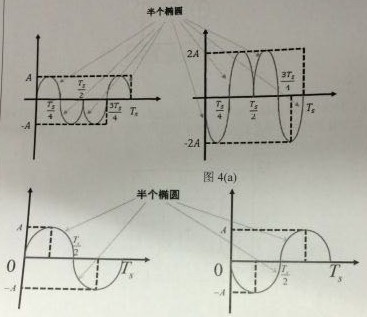
\includegraphics[width=8cm,height=8cm]{3_6.jpeg}
  \caption*{图4}
\end{figure}
根据上述条件,试回答如下问题:\\
(1)上述波形能承载的信息速率是多少?\\
(2)绘制该通信波形的功率谱,若存在线谱请注意标识。该通信波形带限吗?\\
(3)针对这一通信波形,设计其接收机结构,要求尽可能简单,并需详细说明其匹配滤波器的位置及其数学
表达式;\\
(4)计算该通信信号的每符号能量和平均功率;\\
以下第(5、6、7),可以选两种做法。\\
做法一:做(5)(6)。\\
做法二:做(7)。\\
(5)写出其等效基带模型,给出符号集合的数学表达式及其直观表示:(提示:类似星座图)\\
(6)在你画出的类似星座图上给出最佳判决门限(需有数学表达式),并计算其误符号率和误bit率。\\
(7)求出最佳接收时I路和Q路的误比特率及总误符号率。\\
(8)若允许基于该调制方式和硬判决(即(6)中的判决方式)进行信道编码,则最大的可靠的传输速率是
多少?\\
(9)若改变I路的判决方式,允许接收机对于某些接收符号判为“无法判定”(判为空),且“无法判定”的概率
等于误符号率(即左、右波形误判为对方的概率)的0.5倍,试重新给出最优判决方法,并重做(7);\\
(10)若接收机把A误认为1.05A,试重做(6)-(8);\\
(11)若接收机对载波的相位估计有$\theta=\frac{\pi}{100}$的误差,试重做(5)-(9)。\\
\begin{figure}[H]
  \centering
  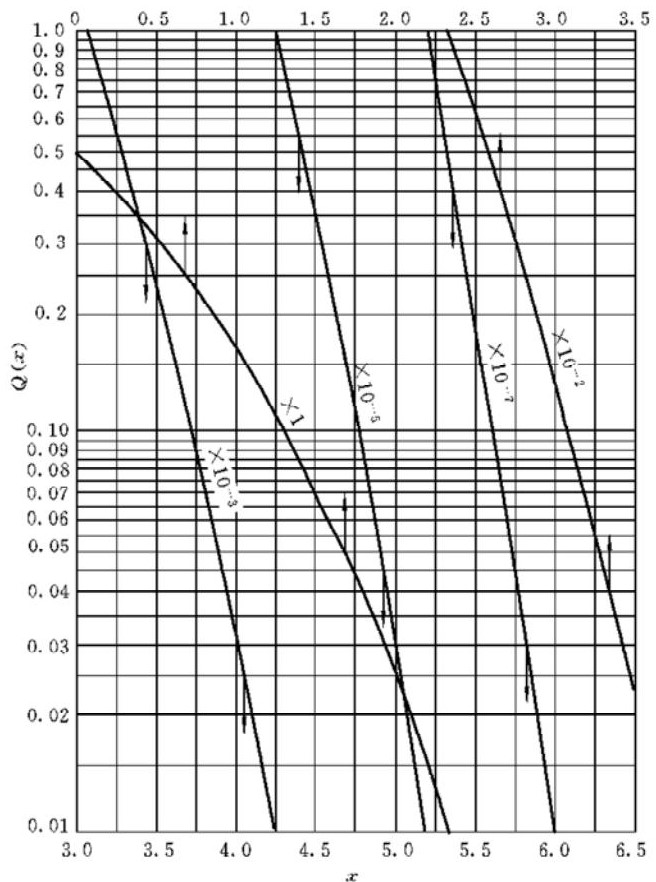
\includegraphics[width=15cm,height=20cm]{3_5.jpg}
  \caption*{Q函数图}
\end{figure}
\end{document}